
\documentclass{article} % For LaTeX2e
\usepackage{iclr2027_conference,times}

% Optional math commands from https://github.com/goodfeli/dlbook_notation.
\input{math_commands.tex}

\usepackage{amssymb}
\usepackage{hyperref}
\usepackage{url}
\usepackage{booktabs}
\usepackage{graphicx}
\usepackage{cleveref}

\newcommand{\kamil}[1]{{\color{orange}#1}}
\newcommand{\ls}[1]{{\color{red}{LS: #1}}}
\newcommand{\alek}[1]{{\color{purple}{alek: #1}}}

\title{Learning to Walk Backwards: \\Improving Inversion-based Editing with Low-Rank Adaptation \kamil{We should work on this}}

% Authors must not appear in the submitted version. They should be hidden
% as long as the \iclrfinalcopy macro remains commented out below.
% Non-anonymous submissions will be rejected without review.

\author{Antiquus S.~Hippocampus, Natalia Cerebro \& Amelie P. Amygdale \thanks{ Use footnote for providing further information
about author (webpage, alternative address)---\emph{not} for acknowledging
funding agencies.  Funding acknowledgements go at the end of the paper.} \\
Department of Computer Science\\
Cranberry-Lemon University\\
Pittsburgh, PA 15213, USA \\
\texttt{\{hippo,brain,jen\}@cs.cranberry-lemon.edu} \\
\And
Ji Q. Ren \& Yevgeny LeNet \\
Department of Computational Neuroscience \\
University of the Witwatersrand \\
Joburg, South Africa \\
\texttt{\{robot,net\}@wits.ac.za} \\
\AND
Coauthor \\
Affiliation \\
Address \\
\texttt{email}
}

% The \author macro works with any number of authors. There are two commands
% used to separate the names and addresses of multiple authors: \And and \AND.
%
% Using \And between authors leaves it to \LaTeX{} to determine where to break
% the lines. Using \AND forces a linebreak at that point. So, if \LaTeX{}
% puts 3 of 4 authors names on the first line, and the last on the second
% line, try using \AND instead of \And before the third author name.

\newcommand{\fix}{\marginpar{FIX}}
\newcommand{\new}{\marginpar{NEW}}

%\iclrfinalcopy % Uncomment for camera-ready version, but NOT for submission.
\begin{document}


\maketitle

\begin{abstract}
Diffusion inversion maps an input image to a noise that enables reconstruction and editing. Standard DDIM inversion, however, relies on a local approximation that reuses model predictions across consecutive trajectory states, accumulating error and imprinting spatially correlated image structure into the recovered noise. We introduce a lightweight LoRA adapter that corrects this approximation exclusively during inversion, leaving the original generation pipeline unchanged. With a detailed evaluation on existing benchmarks we show that thanks to the corrected noise recovered by our method, which better matches the Gaussian prior, we can achieve state-of-the-art performance in downstream tasks such as edition or style transfer.

\end{abstract}



\section{Introduction}

Diffusion models have demonstrated unprecedented capabilities in image generation~\citep{sohl2015deep, dhariwal2021diffusion}, but manipulating existing images remains a significant challenge. Because diffusion generation relies on a multi-step iterative process rather than a well-behaved latent space, editing an existing image first requires inversion -- mapping the image back to an initial noise vector. A perfectly recovered noise representation is critical, as it serves as the foundation for any subsequent structural or stylistic modifications.

A common approach to inversion is based on Denoising Diffusion Implicit Models (DDIM)~\citep{song2020denoising}, which define generation as a deterministic trajectory and therefore allow the process to be approximately reversed to recover the initial noise. However, the reverse update used by standard DDIM inversion is not an exact inverse of the forward process. Instead, it relies on a local linear approximation that reuses the model's noise prediction across consecutive timesteps. This approximation introduces an error at each inversion step, causing the recovered trajectory to progressively diverge from the one followed during generation. As a result, the recovered latent does not faithfully resemble the underlying Gaussian noise, but retains spatially correlated structure from the input image~\citep{staniszewski2026there}. 
% These correlations can be particularly apparent in otherwise homogeneous regions, where the inverted noise exhibits patterns that are absent from an unstructured Gaussian prior. 
Such deviations can compromise the suitability of the inverted latent for subsequent image editing, since image content becomes entangled with the representation intended to encode noise. Existing approaches often address the resulting reconstruction errors through additional correction or stabilization mechanisms~\citep{}\kamil{CITE smth}, but the underlying trajectory mismatch remains inherent to the standard inversion procedure.

In this work, we propose to exactly solve the error introduced by DDIM inversion by directly adapting the model to align with its true trajectory predictions. We introduce a lightweight, trajectory-supervised LoRA adapter that corrects the linear approximation exclusively during the inversion phase. Our approach maps cleaner latents to the exact noise predictions required to recover the preceding, noisier points in the trajectory. Because this adapter is applied solely during inversion, the original generation pipeline remains entirely unchanged. Furthermore, our method is highly efficient: it requires only LoRA finetuning on trajectories from sample generations, relies on no external data, and introduces zero additional inference costs.

By fundamentally correcting the inversion trajectory, our simple technique successfully removes spatial correlations from the observed latents, resulting in recovered noise that rigorously matches the theoretical prior. This foundational correction guarantees superior baseline editability. Through extensive evaluation on existing benchmarks, we demonstrate that delivering mathematically clean latents to existing downstream editors yields state-of-the-art stability and consistent performance gains in tasks such as style transfer and structural editing, proving that better inversion natively unlocks better editing.

Our contribution can be summarized as follows:

\begin{itemize}
    \item We introduce a lightweight, trajectory-supervised LoRA adapter that corrects DDIM linear approximation errors introduced during inversion
    \item We demonstrate that this exact trajectory alignment successfully eliminates spatial correlations from the inverted latents, recovering unstructured noise that faithfully matches the theoretical Gaussian prior.
   
    \item We show that correcting the inversion space yields state-of-the-art stability and performance in downstream editing tasks, achieving this with zero external training data and no additional inference overhead.
     \alek{This overstates the results a bit - we don't have full SOTA in downstream tasks}
\end{itemize}

% \begin{itemize}
%     \item Diffusion is cool, but it's not that easy to edit images with diffusion model because of many steps, no latent space etc.
%     \item Inversion allows us to go back to the initial noise but as noticed by recent works it introduces some errors
%     \item This error can be mostly attributed to the linear assumption
%     \item Most of the existing works for image edition focus on adding some tricks to stabilize the reconstruction
%     \item We propose to exactly solve the issue introduced by the DDIM inversion by simply adapting the model to align with the true predictions from the model
%     \item We then can use this adapter only for inversion, while keeping the model intact
%     \item We show that our simple technique allows us to completely remove correlations from the observed latents, what leads to superior editability of the inverted latents
%     \item Importantly our method is cheap as it requires only LoRA finetuning on the trajectories from the samples generations, so it requires no data, and introduces no additional inference costs.
% \end{itemize}


\section{Background \& related work}
\label{sec:background}

\paragraph{Diffusion models.} The diffusion framework formulates the generative process as a transition between two distributions: training data $\mathcal{X}$ (e.g., image and audio samples) and Gaussian $\mathcal{N}(0,\mathcal{I})$. 
Diffusion Models (DMs) are trained to denoise samples, i.e., to reverse a process of gradually corrupting data with noise, referred as \textit{forward diffusion}. Given a pair of samples $\big(x_0\sim X;\epsilon\sim\mathcal{N}(0,\mathcal{I})\big)$ from both distributions, such a process interpolates between them as  
\begin{equation}\label{eq:forward}
    x_t=\sqrt{\bar{\alpha}_t}\,x_0+\sqrt{1-\bar{\alpha}_t}\,\epsilon,
\end{equation} given
$\bar{\alpha}_t=\prod_{s=1}^{t}\alpha_s$ and $\alpha_t=1-\beta_t$, where $\{\beta_t\}_{t=1}^{T}$ is a variance schedule, describing decreasing signal-to-noise ratio (SNR) of data. 

For Denoising Diffusion Implicit Models (DDIMs, \citet{song2020denoising}), the reverse process starts from independent random noise $x_T\sim\mathcal{N}(0,\mathcal{I})$ and prompt conditioning $c$ and produces a clean sample $x_0$ by iteratively (in steps $t=T\dots1$) subtracting the noise predicted by trained model $\eps_\theta$:
\begin{equation}\label{eq:ddim-gen-process}
    x_{t-1} = \frac{1}{\sqrt{\alpha_{t}}}\cdot x_t - (\frac{\sqrt{1-\bar{\alpha}_t}}{\sqrt{\alpha_t}}-\sqrt{1-\bar{\alpha}_{t-1}})\cdot\epsilon_\theta(x_t,t,c).
\end{equation}

Notably, this process of obtaining a less noisy sample from a more noisy one is deterministic, offering a fixed noise--data mapping. Such determinism makes the generative process reversible in principle: any arbitrary image or audio can be encoded back to its corresponding noise by rearranging terms in \cref{eq:ddim-gen-process} and running it backward in time ($t=1\dots T$):
\begin{equation}\label{eq:ddim-inv-noapprox}
    x_t=\sqrt{\alpha_t}\,x_{t-1}+\left(\sqrt{1-\bar{\alpha}_t}-\sqrt{\alpha_t-\bar{\alpha}_t}\right)\cdot\epsilon_\theta(x_t,t,c).
\end{equation}
This process, referred to in literature as \textit{inversion}, builds the foundation for methods designed for tasks such as editing \citep{}, style transfer \citep{}, or generative content watermarking \citep{}. However, directly applying the update from \cref{eq:ddim-inv-noapprox} is infeasible, since computing $x_t$ requires the model prediction at $x_t$ itself. Thus, standard DDIM Inversion~\citep{dhariwal2021diffusion} resolves this circular dependency through local approximation, evaluating the model at the available (cleaner) state instead:
\begin{equation}\label{eq:ddim-inv-approx}
    \epsilon_\theta(x_t,t,c)\approx\epsilon_\theta(x_{t-1},t,c).
\end{equation}

Recent studies have analyzed the consequences of this approximation. Accumulated over a sequence of steps, it causes the recovered noise to deviate statistically from the Gaussian prior and entangle the structure of the input image~\citep{parmar2023zero,garibi2024renoise,lin2024schedule,staniszewski2026there,jiao2026unieditflow} or significantly degrade downstream editing, especially when employed in settings with a higher guidance score \citep{ho2021classifierfree, Mokady_2023_CVPR}. \citet{staniszewski2026there} trace the problem to approximation error at the first inversion steps at low-frequency image areas, whereas \citet{lin2024schedule} attribute it to the singularity problem in the noise schedule. 

\paragraph{Inversion methods.}
Despite its approximation error, DDIM inversion forms the basis for numerous applications, including inpainting~\citep{DBLP:conf/icml/ZhangJZYJC23}, interpolation~\citep{dhariwal2021diffusion,zheng2024noisediffusion}, style transfer~\citep{}, and editing~\citep{su2022dual,Kim_2022_CVPR,hertz2022prompttoprompt,Ceylan_2023_ICCV,Deja2023}. A large body of work improves inversion for text-to-image models, where classifier-free guidance further amplifies the inversion error~\citep{Mokady_2023_CVPR,garibi2024renoise,huberman2024edit,meiri2023fixed,hong2024exact,miyake2023negativeprompt,han2024proxedit,dong2023prompt,NEURIPS2023_61960fdf,parmar2023zero,iterinv,wallace2023edict,Pan_2023_ICCV,wang2024belm0,brack2023ledits,lin2024schedule,ju2024pnp}. 
One family optimizes the conditioning: Null-text inversion~\citep{Mokady_2023_CVPR} tunes the null embedding at each step to reduce reconstruction error, and related methods search for prompt embeddings~\citep{miyake2023negativeprompt,han2024proxedit,dong2023prompt}. 
A second family applies numerical schemes at inference time: fixed-point iteration~\citep{meiri2023fixed,Pan_2023_ICCV}, exact inversion of higher-order solvers~\citep{hong2024exact}, bidirectional-explicit multistep updates~\citep{wang2024belm0}, or auxiliary coupled trajectories~\citep{wallace2023edict}. In particular, ReNoise~\citep{garibi2024renoise} iteratively re-estimates each trajectory point by averaging successive noise predictions and regularizes patch-level correlations to keep the latents editable, while \citet{parmar2023zero} directly regularize the inversion output toward Gaussian statistics. 
A third group compensates for the error downstream: Direct Inversion~\citep{ju2024pnp} records the per-step deviation between the inversion and reconstruction trajectories and re-adds it during editing. 
Finally, some works change the process being inverted: \citet{huberman2024edit}, followed by \citet{brack2023ledits}, invert the stochastic DDPM sampler by extracting its per-step noise maps, 
\citet{staniszewski2026there} and \citet{lin2024schedule} modify the noise schedule to stabilize inversion. 

These approaches either accept the local-linearity approximation of \eqref{eq:ddim-inv-approx} and compensate for its consequences, or pay for exactness with additional model evaluations or stored state. In contrast, we remove the source of the error directly: a lightweight LoRA adapter, trained on the frozen model's own trajectories, supplies the prediction that the approximation replaces, at no additional inference cost and with the generation process left unchanged.

\paragraph{LoRA.} 

\ls{describe here LoRA + these 2-3 methods that combine it with inversion? \begin{enumerate}
    \item FlashIn: Fast and Accurate Image Inversion for Real-time Image Editing
    \item BiFM: Bidirectional Flow Matching for Few-Step Image Editing and Generation
    \item DeepInv: A Novel Self-supervised Learning Approach for Fast and Accurate Diffusion Inversion
2\end{enumerate}}

\section{Method}
We apply the diffusion process introduced in Section~\ref{sec:background} in the latent space of a pretrained model, so every state $x_t$ below denotes a VAE latent rather than an image in pixel space. Let $\epsilon_\theta$ be the frozen noise predictor and let $\phi$ denote the parameters of a low-rank adaptation applied to its denoising network. We write the adapted predictor as
\[
\epsilon_{\theta,\phi}(x,t,c)
=
\epsilon_\theta(x,t,c)
+
\Delta_\phi(x,t,c),
\]
where $\Delta_\phi$ denotes the change in the network prediction induced by the internal LoRA weight updates, $t$ is a diffusion timestep, and $c$ is the text conditioning. The adapter learns to map an available cleaner latent to the noise prediction required to recover its adjacent noisier trajectory state.

\subsection{Trajectory-Supervised LoRA Inversion}
\label{sec:trajectory-objective}
We construct the training set from deterministic DDIM sampling trajectories generated by the base model. Let $t_0>t_1>\cdots>t_{N-1}$ denote the $N$ model-evaluation timesteps in generation order, and let $t_N$ denote the terminal clean endpoint associated with the scheduler's final cumulative coefficient. Thus, $x_{t_i}$ is noisier than the adjacent state $x_{t_{i+1}}$, generation traverses the trajectory from $i=0$ to $N-1$, and inversion traverses it in the opposite direction. For a generation transition, the frozen model produces the teacher prediction

\[ \epsilon_i^{\mathrm{teach}}=\epsilon_\theta(x_{t_i},t_i,c), \]

which is then used by the deterministic DDIM update to obtain $x_{t_{i+1}}$. This teacher prediction is the frozen model output at the correct noisy trajectory state; it is not the Gaussian noise used to initialize the trajectory.

During inversion, $x_{t_i}$ is unknown. Applying the local approximation in Eq.~\eqref{eq:ddim-inv-approx} to scheduler transition $i$ evaluates the frozen denoiser at the available cleaner state while retaining the noisy-endpoint timestep, giving $\tilde{\epsilon}_i^{\mathrm{DDIM}}=\epsilon_\theta(x_{t_{i+1}},t_i,c)$. Our adapter instead learns the unavailable trajectory prediction directly. Given $x_{t_{i+1}}$ and $t_i$, it produces $\hat{\epsilon}_i=\epsilon_{\theta,\phi}(x_{t_{i+1}},t_i,c)$ and is supervised by $\epsilon_i^{\mathrm{teach}}$:

\[ \mathcal{L}_{\mathrm{inv}}=\mathbb{E}_{(x_{t_i},x_{t_{i+1}},t_i,c)}\left[\left\|\epsilon_{\theta,\phi}(x_{t_{i+1}},t_i,c)-\epsilon_i^{\mathrm{teach}}\right\|_2^2\right]. \]

The squared error is averaged over latent elements and sampled transitions. To recover the predicted noisy endpoint for an arbitrary gap in the sampling schedule, we first form the corresponding clean-latent prediction and then evaluate it at the noisier schedule coefficient:

\[ \hat{x}_0^{(i)}=\frac{x_{t_{i+1}}-\sqrt{1-\bar{\alpha}_{t_{i+1}}}\,\hat{\epsilon}_i}{\sqrt{\bar{\alpha}_{t_{i+1}}}}, \qquad \hat{x}_{t_i}=\sqrt{\bar{\alpha}_{t_i}}\,\hat{x}_0^{(i)}+\sqrt{1-\bar{\alpha}_{t_i}}\,\hat{\epsilon}_i. \]

Because $x_{t_{i+1}}$ was generated deterministically from $x_{t_i}$ using $\epsilon_i^{\mathrm{teach}}$, substituting $\hat{\epsilon}_i=\epsilon_i^{\mathrm{teach}}$ into this inverse update recovers $\hat{x}_{t_i}=x_{t_i}$, assuming the same scheduler and no clipping or thresholding. We train by uniformly sampling adjacent transitions from the saved trajectories. Each training example contains the cleaner latent $x_{t_{i+1}}$, the noisy-endpoint timestep $t_i$, prompt conditioning $c$, and the cached teacher target $\epsilon_i^{\mathrm{teach}}$.

\subsection{Cycle-Consistent Regularization}
\label{sec:cycle-objective}
The inversion objective supervises the adapter in prediction space, but it does not directly measure whether the resulting inverted state can be mapped back to the cleaner trajectory state by the frozen generation process. With finite prediction error, inversion may produce an off-trajectory state $\hat{x}_{t_i}$, causing the frozen denoiser to be evaluated at this predicted state rather than at the saved state $x_{t_i}$. We therefore introduce a one-transition cycle that measures the downstream effect of this error in latent space.

Let $I_{i,\theta,\phi}(\cdot;c)$ denote the LoRA-enabled inverse update from $t_{i+1}$ to $t_i$, and let $G_{i,\theta}(\cdot;c)$ denote the frozen DDIM generation update over the same interval. Starting from $x_{t_{i+1}}$, we obtain $\hat{x}_{t_i}=I_{i,\theta,\phi}(x_{t_{i+1}};c)$, disable the adapter, recompute the noise prediction at $\hat{x}_{t_i}$ with the frozen base model, and generate $\tilde{x}_{t_{i+1}}=G_{i,\theta}(\hat{x}_{t_i};c)$. The cycle loss is

\[ \mathcal{L}_{\mathrm{cycle}}=\mathbb{E}_{(x_{t_{i+1}},t_i,c)}\left[\left\|G_{i,\theta}\!\left(I_{i,\theta,\phi}(x_{t_{i+1}};c);c\right)-x_{t_{i+1}}\right\|_2^2\right]. \]

This objective is consistent with the inversion loss: if $\hat{\epsilon}_i=\epsilon_i^{\mathrm{teach}}$, then $\hat{x}_{t_i}=x_{t_i}$ and the frozen generation transition maps it exactly back to $x_{t_{i+1}}$, making $\mathcal{L}_{\mathrm{cycle}}=0$.

The cycle-regularized variant optimizes

\[ \mathcal{L}_{\mathrm{total}}=\mathcal{L}_{\mathrm{inv}}+\lambda_{\mathrm{cycle}}\mathcal{L}_{\mathrm{cycle}}, \]

where $\lambda_{\mathrm{cycle}}\geq0$ controls the regularizer and $\lambda_{\mathrm{cycle}}=0$ recovers the core trajectory-supervised objective. The parameters $\theta$ remain frozen throughout training, including during the generation half of the cycle. We nevertheless retain gradients with respect to the input $\hat{x}_{t_i}$, allowing the cycle error to propagate through the frozen denoiser and both DDIM updates to the LoRA parameters $\phi$.

\subsection{Integration with Direct Inversion}
At inference time, the adapter is enabled only while constructing the source inversion trajectory and is disabled before reconstruction or editing. In the standalone variant, the LoRA-generated trajectory directly replaces the conventional DDIM inversion trajectory supplied to the downstream editor. In the fused LoRA+DirectInv variant, we modify only the first stage of Direct Inversion: its initial DDIM trajectory is replaced with our LoRA inversion trajectory. The subsequent Direct Inversion corrections and the complete editor-specific reverse process remain unchanged and use the original frozen model without the adapter.


\subsection{Inversion with Classifier-Free Guidance}
\alek{We need to keep consistent math notation across sections}
\label{sec:method-extensions}
\label{sec:guided-objective}

\paragraph{Guided trajectory supervision.}
Classifier-free guidance (CFG) combines unconditional and conditional noise
predictions~\citep{ho2021classifierfree}:
\begin{equation}
 \epsilon_\theta^w(z,\tau,c)
 =(1-w)\epsilon_\theta(z,\tau,\varnothing)
 +w\epsilon_\theta(z,\tau,c).
 \label{eq:guided-prediction}
\end{equation}
At $w=1$, only the conditional prediction contributes. For $w>1$, correcting
that branch alone does not constrain the unconditional contribution to the
inverse update. We therefore extend trajectory supervision to the predictions
that actually enter the guided DDIM operator.

For each adjacent transition generated by the frozen model at guidance $w$,
we cache both teacher predictions at the noisier state $z_i$:
$e_i^u=\epsilon_\theta(z_i,\tau_i,\varnothing)$ and
$e_i^c=\epsilon_\theta(z_i,\tau_i,c)$.
The composed teacher is $e_i^w=(1-w)e_i^u+w e_i^c$.
Both student branches instead receive the cleaner state $z_{i+1}$, while
retaining the same noisy-endpoint timestep $\tau_i$ and conditioning:
$\hat e_i^u=\epsilon_{\theta,\phi_u}(z_{i+1},\tau_i,\varnothing)$ and
$\hat e_i^c=\epsilon_{\theta,\phi_c}(z_{i+1},\tau_i,c)$.
\alek{Comment}
Thus the learned correction addresses the change of evaluation state, rather
than a change of timestep or prompt. The teacher composition uses the guidance
that generated the saved transition; in mixed-guidance training, this value
is attached to each example.

\paragraph{Adapter sharing and training objectives.}
We compare two independent design choices. A \emph{shared} adapter uses
$\phi_u=\phi_c=\phi$, whereas a \emph{pair} uses separate trainable adapters
for the two branches of the same frozen backbone. Either parameterization can
optimize the composed CFG prediction or the individual branches:
\begin{align}
 \mathcal{L}_{\mathrm{CFG}}
 &=\mathbb{E}\!\left[
 \left\|(1-w)\hat e_i^u+w\hat e_i^c-e_i^w\right\|_2^2\right],
 \label{eq:cfg-composed-loss}\\
 \mathcal{L}_{\mathrm{branch}}
 &=\mathbb{E}\!\left[
 \left\|\hat e_i^u-e_i^u\right\|_2^2
 +\left\|\hat e_i^c-e_i^c\right\|_2^2\right].
 \label{eq:cfg-branch-loss}
\end{align}
The implementation averages squared errors over tensor elements and training
examples; the branch objective sums the two branch means. These choices give
the shared CFG, shared branch, pair CFG, and pair branch variants reported in
Section~\ref{sec:cfg-experiments}. Only adapter parameters are optimized.
\subsection{Flow Matching}
\label{sec:flow-objective}

We extend the trajectory-supervised objective of
Section~\ref{sec:trajectory-objective} to flow-matching models by learning
the velocity prediction required by an Euler inverse step. Let $v_\theta$
denote the pretrained and frozen velocity model and $v_{\theta,\phi}$ its
LoRA-adapted counterpart. We apply this formulation to FLUX.1-dev~\citep{flux},
which takes text conditioning $c$ and an embedded guidance value $g$.
\alek{Comment}
Here $g$ is an input to the transformer, rather than a coefficient used to
combine conditional and unconditional predictions.

We construct the training set from Euler sampling trajectories generated by
the base model. Following the indexing above, $z_i$ is the noisier state and
$z_{i+1}$ is the adjacent cleaner state. Let $\sigma_i>\sigma_{i+1}$ be their
noise levels, $h_i=\sigma_i-\sigma_{i+1}$ the interval size, and $\tau_i$ the
model timestep at the noisy endpoint. The intervals follow the model's
sampling schedule and need not be uniform. For each transition, the frozen
model produces the teacher velocity
\[
 v_i^{\mathrm{teach}}=v_\theta(z_i,\tau_i,c,g),
\]
which is used in the Euler sampling update
\begin{equation}
 z_{i+1}=z_i-h_i v_i^{\mathrm{teach}}.
 \label{eq:flow-forward-step}
\end{equation}

During inversion, $z_i$ is unknown. Standard Euler inversion therefore
replaces the unavailable teacher velocity with a prediction at the cleaner
state, retaining the same noisy-endpoint timestep:
\[
 \tilde v_i^{\mathrm{Euler}}=v_\theta(z_{i+1},\tau_i,c,g)
 \approx v_\theta(z_i,\tau_i,c,g).
\]
As in DDIM inversion, this approximation evaluates the model at a different
state from the one used to generate the transition. Our adapter learns the
missing trajectory prediction from the state available during inversion.
Given $z_{i+1}$ and $\tau_i$, it produces
$\hat v_i=v_{\theta,\phi}(z_{i+1},\tau_i,c,g)$ and is supervised by the
cached teacher velocity:
\begin{equation}
 \mathcal{L}_{\mathrm{vel}}
 =\mathbb{E}_{(z_i,z_{i+1},\tau_i,c,g)}\left[
 \left\|v_{\theta,\phi}(z_{i+1},\tau_i,c,g)
       -v_i^{\mathrm{teach}}\right\|_2^2\right].
 \label{eq:flow-objective}
\end{equation}
Teacher and student use the same timestep, text conditioning, and embedded
guidance; only their latent inputs differ. We optimize attention LoRA in
the FLUX transformer while keeping the base parameters frozen. Squared
errors are averaged over latent elements and sampled transitions. The
reported FLUX adapters use this velocity objective without cycle
regularization ($\lambda_{\mathrm{cycle}}=0$), with separate adapters
trained for each source-guidance setting.

The predicted velocity enters the inverse update as
\begin{equation}
 \hat z_i=z_{i+1}+h_i\hat v_i.
 \label{eq:flow-inverse-step}
\end{equation}
\alek{Comment}
Because $z_{i+1}$ was generated from $z_i$ using $v_i^{\mathrm{teach}}$,
substituting $\hat v_i=v_i^{\mathrm{teach}}$ recovers $\hat z_i=z_i$
for the same saved transition and interval, up to numerical and stored
precision. Thus the cached velocity provides the target needed to reverse
each Euler sampling step, analogously to the cached noise prediction in
Section~\ref{sec:trajectory-objective}.

At inference time, we start from the image latent and traverse the schedule
towards noise. At each step, the adapted model receives the current inverse
state and predicts the velocity for the next update. LoRA is enabled only
during inversion; reconstruction and editing use the frozen base
transformer. Section~\ref{sec:flux-experiments} reports the training and
evaluation guidance settings, including comparisons with different guidance
values for inversion and generation.

\section{Experiments}

\subsection{Experimental setup}
We evaluate the proposed inversion correction across noise recovery and image reconstruction, text-guided image editing, style transfer, music editing, and flow-matching models. Throughout these experiments, the adapter is enabled only during inversion; reconstruction and editing use the corresponding frozen base model and unchanged downstream method. The image adapters are trained on deterministic 50-step trajectories synthesized by the respective frozen backbone from ReCap-COCO prompts, without using benchmark images. We evaluate LoRA ranks $8$, $16$, and $32$ and train separate adapters for SDXL and Stable Diffusion 1.5. The following subsections describe the task-specific protocols, while Appendix~\ref{sec:implementation-details} provides complete training and implementation details.

\subsection{Inversion quality}
We isolate inversion quality on a held-out set of 1,522 ReCap-COCO prompts. For each prompt, Stable Diffusion XL generates a reference trajectory and image at $1024\times1024$ resolution using 50 deterministic DDIM steps and classifier-free guidance (CFG) scale $1$. Because the initial noise is known, we can evaluate both recovery of that noise and reconstruction of the generated reference image. We compare standard DDIM inversion, our LoRA inversion, and the forward-diffusion correction of \citet{staniszewski2026there} under the same prompts, seeds, scheduler, and conditioning. Forward $2\%$ and Forward $4\%$ replace, respectively, the first one and two of the 50 inversion updates closest to the clean-image latent with closed-form forward-diffusion updates. Reconstruction always uses the frozen base model without the adapter.

Table~\ref{tab:inversion-quality} evaluates both recovery of the known initial noise and reconstruction of the generated reference image. Correlation is the mean top-$k$ Pearson correlation within $8\times8$ latent patches, and KL is the Gaussian divergence between the recovered and original noise distributions. Our learned correction improves both sides of the normality--fidelity trade-off: increasing rank monotonically lowers correlation and KL while also lowering MAE and LPIPS and increasing PSNR and SSIM. In particular, $r=32$ improves PSNR from the DDIM regime to $30.40$ and reduces KL by more than an order of magnitude.
\begin{table*}[t]
    \centering
    \small
    \caption{Comparison of standard DDIM inversion, the forward-diffusion correction of \citet{staniszewski2026there}, and our trajectory-supervised LoRA inversion on SDXL. Correlation and KL divergence assess recovered-noise normality, while MAE, LPIPS, PSNR, and SSIM assess image reconstruction. Bold denotes the best result.}
    \label{tab:inversion-quality}
    \resizebox{\textwidth}{!}{%
    \begin{tabular}{lrrrrrr}
        \toprule
        Method & Corr. \(\downarrow\) & KL Div. \(\times10^2\) \(\downarrow\) & MAE \(\downarrow\) & LPIPS \(\downarrow\) & PSNR \(\uparrow\) & SSIM \(\uparrow\) \\
        \midrule
        DDIM Inv.       & 0.17 & 0.71 & 0.03 & 0.10 & 28.22 & 0.81 \\
        Forward \(2\%\) & 0.15 & 0.54 & 0.03 & 0.10 & 27.69 & 0.79 \\
        Forward \(4\%\) & 0.11 & 0.24 & 0.04 & 0.14 & 25.84 & 0.70 \\
        \midrule
        LoRA \(r=8\)  & 0.10 & 0.08 & 0.02 & 0.06 & 30.06 & 0.87 \\
        LoRA \(r=16\) & 0.10 & 0.07 & 0.02 & 0.06 & 30.22 & 0.87 \\
        LoRA \(r=32\) & \textbf{0.10} & \textbf{0.05} & \textbf{0.02} & \textbf{0.06} & \textbf{30.40} & \textbf{0.87} \\
        \bottomrule
    \end{tabular}}
\end{table*}
\begin{figure}[t]
    \centering
    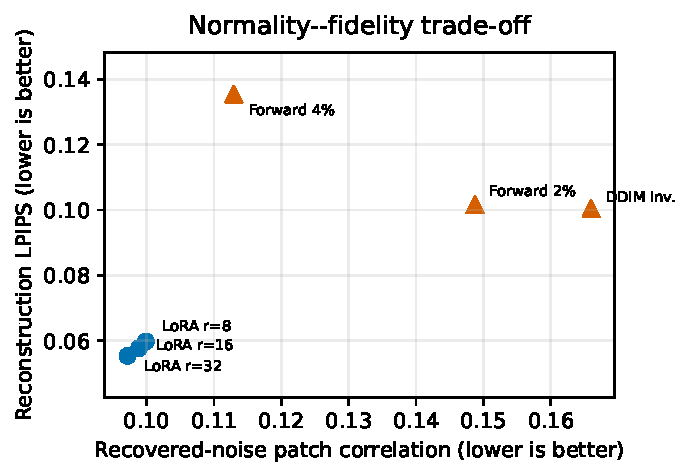
\includegraphics[width=0.72\linewidth]{figures/inversion_normality_fidelity.pdf}
    \caption{Normality--fidelity trade-off between spatial correlation in the recovered noise and perceptual reconstruction error. Lower and further left is better.}
    \label{fig:inversion-pareto}
\end{figure}

The forward-diffusion correction reduces spatial correlation by injecting independent noise, but stronger replacement also sacrifices reconstruction fidelity. In contrast, full-trajectory LoRA moves toward the lower-left of Figure~\ref{fig:inversion-pareto}: it removes structured residuals while preserving information needed by the unchanged reverse process. Appendix~\ref{sec:extended-inversion} reports rank, active-step, regional, text-editing, and CFG ablations.
\subsection{PieBench editing benchmark}
We evaluate DDIM, Direct Inversion, LoRA, and LoRA+DirectInv on all 700 PIE-Bench examples using Stable Diffusion 1.5 and four editors: Prompt-to-Prompt (P2P), Plug-and-Play (PnP), MasaCtrl, and Pix2Pix-Zero. Structure measures global consistency, PSNR, LPIPS, MSE, and SSIM measure preservation in the unedited region, and the two CLIP scores measure target-prompt alignment over the full image and edited region. Complete inference settings, mask handling, and configuration-selection details are provided in Appendix~\ref{sec:evaluation-protocol}.

Table~\ref{tab:sd15-four-way-inversion} compares the reproduced controls with selected configurations from each LoRA training family. For P2P, cycle-consistent LoRA+DirectInv substantially improves every preservation metric over DirectInv, while standalone LoRA gives the strongest CLIP scores. PnP and MasaCtrl exhibit a trade-off: DirectInv retains the strongest preservation, whereas LoRA-based configurations improve text alignment. Pix2Pix-Zero shows the same split. Final-tail $r=8$ gives the highest CLIP target score, while cycle-consistent $r=32$ gives the highest CLIP edit score; neither improves its preservation metrics over DirectInv.
\kamil{Can you find a few nice examples, where it works? :) + please copy paste those results for just reconstruction}
\begin{figure}
    \centering
    \includegraphics[width=0.7\linewidth]{figures/qualitative/directinv_lora_qualitative_comparison_images_only.png}
    \caption{Qualitative PIE-Bench comparison of SD1.5 DirectInv and LoRA+DirectInv (ours). Columns show the source, DirectInv, and ours; rows show P2P (dog to monkey), PnP (facial tattoo), MasaCtrl (remove laptop), and Pix2Pix-Zero (round to square cake). LoRA is used only during inversion.}
    \label{fig:pie_bench_results}
\end{figure}
\begin{table*}[t]
  \centering
  \scriptsize
  \setlength{\tabcolsep}{2.5pt}
  \renewcommand{\arraystretch}{0.92}
  \caption{PIE-Bench editing with SD1.5. Bold denotes the best result within each editor.}
  \label{tab:sd15-four-way-inversion}
  \resizebox{\textwidth}{!}{%
  \begin{tabular}{lll rrrrrrr}
    \toprule
    Editor & Inversion & Training &
    Structure ($\times 10^3$) $\downarrow$ & PSNR $\uparrow$ &
    LPIPS ($\times 10^3$) $\downarrow$ & MSE ($\times 10^4$) $\downarrow$ &
    SSIM ($\times 10^2$) $\uparrow$ & CLIP target $\uparrow$ &
    CLIP edit $\uparrow$ \\
    \midrule
    P2P & DDIM & -- & 70.50 & 17.84 & 210.15 & 220.28 & 71.56 & 25.19 & 22.39 \\
    P2P & DirectInv & -- & 31.35 & 22.57 & 125.51 & 91.27 & 78.54 & 25.07 & 22.22 \\
    P2P & LoRA & uniform $r=8$ & 70.45 & 17.81 & 211.10 & 221.32 & 71.37 & \textbf{25.38} & \textbf{22.57} \\
    P2P & LoRA+DirectInv & uniform $r=8$ & 14.12 & 26.02 & 73.25 & 44.40 & 83.50 & 25.33 & 22.31 \\
    P2P & LoRA+DirectInv & final-tail $r=8$ & 14.27 & 25.95 & 72.48 & 44.31 & 83.55 & 25.35 & 22.37 \\
    P2P & LoRA+DirectInv & cycle $r=16,\lambda=0.5$ & \textbf{14.00} & \textbf{26.05} & \textbf{71.76} & \textbf{43.57} & \textbf{83.60} & 25.28 & 22.31 \\
    \midrule
    PnP & DDIM & -- & 27.32 & 22.31 & 112.76 & 82.98 & 79.58 & 25.59 & 22.57 \\
    PnP & DirectInv & -- & \textbf{23.33} & \textbf{22.46} & \textbf{105.51} & \textbf{79.97} & \textbf{80.22} & 25.63 & 22.67 \\
    PnP & LoRA & uniform $r=32$ & 27.08 & 22.33 & 113.47 & 81.70 & 79.54 & 25.61 & 22.81 \\
    PnP & LoRA+DirectInv & uniform $r=8$ & 24.27 & 22.37 & 110.17 & 81.82 & 79.90 & \textbf{25.83} & 22.85 \\
    PnP & LoRA+DirectInv & final-tail $r=32$ & 24.43 & 22.36 & 110.82 & 81.83 & 79.88 & 25.82 & \textbf{22.89} \\
    PnP & LoRA+DirectInv & cycle $r=8,\lambda=1$ & 24.19 & 22.38 & 110.03 & 81.64 & 79.92 & 25.82 & \textbf{22.89} \\
    \midrule
    MasaCtrl & DDIM & -- & 27.68 & 22.32 & 105.51 & 84.69 & 80.41 & 24.16 & 21.20 \\
    MasaCtrl & DirectInv & -- & \textbf{23.57} & \textbf{22.82} & \textbf{86.83} & \textbf{79.19} & \textbf{82.02} & 24.51 & 21.47 \\
    MasaCtrl & LoRA & uniform $r=16$ & 26.49 & 22.29 & 105.30 & 87.57 & 80.37 & 24.22 & 21.18 \\
    MasaCtrl & LoRA+DirectInv & uniform $r=8$ & 28.58 & 21.90 & 99.01 & 99.13 & 80.49 & 24.61 & \textbf{21.50} \\
    MasaCtrl & LoRA+DirectInv & final-tail $r=8$ & 28.38 & 21.93 & 98.72 & 98.66 & 80.54 & \textbf{24.64} & 21.46 \\
    MasaCtrl & LoRA+DirectInv & cycle $r=16,\lambda=4$ & 28.51 & 21.90 & 98.89 & 98.91 & 80.50 & 24.62 & \textbf{21.50} \\
    \midrule
    Pix2Pix-Zero & DDIM & -- & 64.97 & 20.31 & 177.80 & 150.71 & 74.91 & 22.97 & 20.69 \\
    Pix2Pix-Zero & DirectInv & -- & \textbf{49.99} & \textbf{21.47} & \textbf{142.46} & \textbf{133.49} & \textbf{77.49} & 23.53 & 21.09 \\
    Pix2Pix-Zero & LoRA & uniform $r=8$ & 51.59 & 21.33 & 145.87 & 140.59 & 76.98 & 23.46 & 20.99 \\
    Pix2Pix-Zero & LoRA+DirectInv & uniform $r=16$ & 51.63 & 21.25 & 147.07 & 137.65 & 76.94 & 23.39 & 20.95 \\
    Pix2Pix-Zero & LoRA+DirectInv & final-tail $r=8$ & 51.67 & 21.33 & 144.87 & 135.70 & 77.15 & \textbf{23.56} & 21.01 \\
    Pix2Pix-Zero & LoRA+DirectInv & cycle $r=32,\lambda=1$ & 53.15 & 21.24 & 146.02 & 138.96 & 76.95 & 23.45 & \textbf{21.11} \\
    \bottomrule
  \end{tabular}}
\end{table*}

\subsection{Style Transfer}

\kamil{Same as previously we need plots/table + a few visual samples}

We study three uses of inversion: supplying a reference trajectory to StyleAligned, initializing text-
driven generation in Inversion-InstantStyle, and supplying content/style latents and attention features
to StyleID. Comparisons use a matched control within each pipeline. The text-driven experiments
use StyleBench, whereas StyleID uses its own released content–style image pairs.

We evaluate text-driven style transfer using all 490 reference images from
the public StyleBench dataset introduced by StyleShot~\citep{styleshot},
covering 73 style directories.
We preserve the archive's unequal numbers of references per style rather
than balancing or filtering them by model performance. Each reference is
paired with all 20 official target prompts from Table~5 of the StyleShot
appendix, preserving their wording and order: 12 short object prompts and
eight longer scene descriptions. This gives 9,800 outputs per method.


\subsubsection{Inversion-InstantStyle}

We use Inversion-InstantStyle from the Style-Rank project~\citep{benaroche2024stylerank},
released through its project website and code repository. It augments
InstantStyle~\citep{instantstyle} with an inverted reference latent.
The reference contributes through both its image
features in IP-Adapter and its recovered endpoint $z_T$. IP-Adapter is
disabled during inversion, and the inversion LoRA is disabled during
generation. Before sampling, the endpoint is mixed with independent noise:
\begin{equation}
 z_{\mathrm{start}}=\frac{z_T+s\epsilon}{\sqrt{1+s^2}},
 \qquad \epsilon\sim\mathcal{N}(0,I).
 \label{eq:instantstyle-renoising}
\end{equation}
The parameter $s$ controls added noise: $s=0$ preserves the inverted
endpoint, whereas $s=1$ gives equal coefficients to the recovered endpoint
and fresh noise. Their actual variance contributions need not be equal if
the inverted endpoint is not standard Gaussian

\subsubsection{StyleAligned}

\subsection{Music Editing}
\label{sec:music-editing}

To test whether trajectory-supervised inversion transfers beyond images, we apply the same objective to text-guided music editing with two text-to-audio latent diffusion models: AudioLDM2-large~\citep{audioldm2}, a 16\,kHz $\epsilon$-prediction UNet sampled with DDIM, and Stable Audio Open~\citep{stableaudioopen}, a 44.1\,kHz stereo $v$-prediction diffusion transformer sampled with a first-order ODE solver on its native schedule. In both cases the inverse update is exact given the model prediction at the noisier state, and inversion approximates that prediction from the cleaner state, so the objective of Section~\ref{sec:trajectory-objective} carries over directly; for each model we train an attention-only adapter on deterministic trajectories generated by the frozen backbone, with no external data. Following the protocol of \citet{manor2024zeroshot}, we edit the 35 MusicDelta multitracks from MedleyDB~\citep{medleydb} by inverting the source audio and regenerating with a target caption, reporting a 115-edit split that spans inversion depths of 25--99\% and two target-guidance scales. Preservation is measured by LPAPS~\citep{manor2024zeroshot} and mel-spectrogram PSNR against the source; edit adherence by CLAP~\citep{laionclap} and MuQ-MuLan~\citep{muq} similarity to the target caption.

The adapters again learn their objective, closing about $90\%$ of the approximation gap on both models, and improve held-out real-audio reconstruction by $+1.6$ and $+1.3$\,dB mel PSNR on AudioLDM2 and Stable Audio Open, respectively (paired, $p<0.001$). Editing, however, separates the two models. On Stable Audio Open (Table~\ref{tab:sao-editing}), the adapter improves LPAPS at every tested operating point (mean $-0.057$, $p<0.001$), and from $50\%$ inversion depth upward improves CLAP and mel PSNR simultaneously---moving off the preservation--adherence front rather than trading along it, although the shift is small relative to the range the depth sweep covers (Figure~\ref{fig:music-fronts}, bottom). On AudioLDM2 the front does not move (Figure~\ref{fig:music-fronts}, top): at a matched inference budget of 800 denoiser calls, the DDIM and DDIM+LoRA curves coincide to within $0.02$ LPAPS at every depth and guidance setting. Consistent with this, DDPM inversion~\citep{huberman2024edit,manor2024zeroshot}, which is exact by construction, traces essentially the same front as approximate DDIM inversion on this model. Inversion error is thus not the binding constraint for AudioLDM2 editing, and corrected inversion helps only where the approximation of the inverse update dominates the remaining error.

\begin{figure}[t]
    \centering
    \includegraphics[width=\linewidth]{figures/music_editing_fronts.pdf}
    \caption{Preservation--adherence Pareto fronts for music editing at matched inference budget. Each curve is the non-dominated set of one method's operating points over inversion depth and target-guidance scale; dominated points are shown as faint markers. Error bars are standard errors over 115 edits. On AudioLDM2 (top), the DDIM fronts with and without the inversion LoRA coincide, and exact DDPM inversion traces the same front. On Stable Audio Open (bottom), the adapter shifts the ODE-inversion front toward better preservation at matched adherence.}
    \label{fig:music-fronts}
\end{figure}

\section{Additional experiments}

\subsection{Inversion with CFG}
\label{sec:cfg-experiments}

We compare two guidance regimes: equal CFG during inversion and generation,
and lower inversion CFG while retaining higher generation CFG.
The matched-guidance evaluation covers CFG 2, 3, 4, 5, 7.5 and 10;
the lower-inversion-guidance evaluation covers generation CFG 5, 7.5 and 10
with inversion CFG fixed at 2.

\paragraph{Matched inversion and generation guidance.}
Table~\ref{tab:cfg-matched-mixed} evaluates DDIM and four mixed-CFG-trained
LoRA configurations at matching inversion and generation guidance:
$w_{\rm inv}=w_{\rm gen}\in\{2,3,4,5,7.5,10\}$. Each guidance setting
contains 166--167 examples. Reconstruction compares the source image with
its reconstruction, whereas CLIP evaluates the output of the synthetic
prompt-shift editing probe.

\paragraph{Separating inversion and generation guidance.}
Table~\ref{tab:high-cfg-ablation} compares DDIM using matched inversion and
generation CFG with DDIM using inversion CFG 2. Source generation,
reconstruction and editing retain CFG 5, 7.5 or 10, with 50 steps in each
direction. The two inversion settings share the same source images, prompts
and seeds: 167 examples at CFG 5 and 166 at each other setting.
Editing prompts are shifted by 1.

\subsection{Flow Matching}
\label{sec:flux-experiments}

We evaluate FLUX.1-dev with base Euler inversion, our LoRA trained for inversion and latent nudging introduced by \citet{stableflow} which multiplies the clean input latent before inversion. All methods use 50 inversion steps and 50 steps for each generation pass. Reconstruction uses the source prompt and editing the target prompt; both are performed by the frozen base model.

\paragraph{Evaluation on synthetic FLUX images.}
Table~\ref{tab:flux-synthetic-guidance} evaluates reconstruction and a
controlled editing probe on 1,000 source images at $1024\times1024$, generated
beforehand by FLUX.1-dev from the prompts from Recap-COCO. They are synthetic FLUX
outputs rather than images taken from the COCO dataset. Guidance $g=1$ and $g=3.5$ use separately trained
adapters and separately generated source trajectories. Within each block,
all methods share source latents, prompts and seeds. The synthetic editing
probe shifts target prompts by one position.

\paragraph{Real-image reconstruction and editing.}
We additionally evaluate all 700 PIE-Bench examples at $512\times512$. Embedded guidance
is $g=1$ for inversion, reconstruction and editing. We score the
source-prompt reconstruction over the entire image, background preservation on
the edited output outside the mask, and target-prompt CLIP agreement on the whole edited image and inside the mask.

\kamil{What else do we have? }

\section{Conclusion}

\subsection*{AI use statement}

(This section is \textbf{required} and does not count toward the page limit.)

In this work, we used generative AI tools for [tasks with required disclosure].
We have not used generative AI tools for [other tasks with required disclosure],
and [the rest of the required disclosure tasks] are not applicable to this work.
Additionally, we used generative AI tools for [tasks with recommended
disclosure]. We have reviewed all AI-assisted work. [Elaborate. For example, “we
checked LLM-generated research ideas for potential plagiarism through a manual
literature survey”, “LLM-generated code was verified and tested for correctness
by 2 authors”, etc.]. We take responsibility for the final content of this work,
including text, claims or artifacts produced with the aid of generative AI.

See the ICLR 2027 AI Policy for Authors for more details. This statement should
not be more than 1 page.

\subsection*{Ethics statement}

(This section is \textbf{recommended} and does not count toward the page limit.)

If authors feel that their paper submission raises questions regarding the Code
of Ethics, they are encouraged to include a paragraph of Ethics Statement (at
the end of the main text before references) to address potential concerns where
appropriate. Topics include, but are not limited to, studies that involve human
subjects, practices to data set releases, potentially harmful insights,
methodologies and applications, potential conflicts of interest and sponsorship,
discrimination/bias/fairness concerns, privacy and security issues, legal
compliance, and research integrity issues (e.g., IRB, documentation, research
ethics). This statement should not be more than 1 page.

\subsection*{Reproducibility statement}

(This section is \textbf{recommended} and does not count toward the page limit.)

It is important that the work published in ICLR is reproducible. Authors are
strongly encouraged to include a paragraph-long Reproducibility Statement at the
end of the main text (before references) to discuss the efforts that have been
made to ensure reproducibility. This paragraph should not itself describe
details needed for reproducing the results, but rather reference the parts of
the main paper, appendix, and supplemental materials that will help with
reproducibility. For example, for novel models or algorithms, a link to an
anonymous downloadable source code can be submitted as supplementary materials;
for theoretical results, clear explanations of any assumptions and a complete
proof of the claims can be included in the appendix; for any datasets used in
the experiments, a complete description of the data processing steps can be
provided in the supplementary materials. Each of the above are examples of
things that can be referenced in the reproducibility statement.

\subsubsection*{Author Contributions}
If you'd like to, you may include  a section for author contributions as is done
in many journals. This is optional and at the discretion of the authors.

\subsubsection*{Acknowledgments}
Use unnumbered third level headings for the acknowledgments. All
acknowledgments, including those to funding agencies, go at the end of the paper.


\bibliography{iclr2027_conference}
\bibliographystyle{iclr2027_conference}

\appendix
\section{Training and implementation details}
\label{sec:implementation-details}

\paragraph{Trajectory data.}
ReCap-COCO is used as a source of text prompts; the associated COCO images are not used for training. For SDXL, we generate one trajectory for each of 27,396 training prompts and reserve 1,522 disjoint prompts for inversion-quality evaluation. Each trajectory is sampled at $1024\times1024$ with 50 deterministic DDIM steps, CFG $1$, and an empty negative prompt. For Stable Diffusion 1.5, we use all 30,441 prompts because evaluation is performed on the independent PIE-Bench dataset. We generate one $512\times512$ trajectory per prompt with the same number of steps and guidance setting. The SD1.5 trajectories, conditioning tensors, and teacher targets are stored in float32. Each saved transition contains the adjacent latent states, its timestep and text conditioning, and the frozen model prediction used as the regression target.

\paragraph{LoRA configuration and optimization.}
All backbone, VAE, and text-encoder parameters remain frozen. LoRA is applied to the query, key, value, and output projections of the denoising network, with zero dropout. We use ranks $r\in\{8,16,32\}$ with scaling parameters $\alpha\in\{4,8,16\}$, respectively. Trainable adapter parameters are maintained in float32 and optimized with AdamW using learning rate $5\times10^{-5}$, zero weight decay, gradient clipping at $1$, and a cosine learning-rate schedule. SDXL training uses a bfloat16 backbone, batch size $2$, gradient accumulation over four batches, and 171,225 optimizer updates, corresponding to one pass over the 50 transitions of every training trajectory; the first 1,000 updates are used for warmup. SD1.5 training is performed fully in float32 with batch size $128$, no gradient accumulation, and 11,892 optimizer updates, again corresponding to one pass over all 1,522,050 saved transitions; the first 238 updates are used for warmup.

\paragraph{Training variants.}
The uniform objective samples all 50 trajectory transitions with equal probability. The final-tail variant keeps the same number of draws but assigns half of them to the final 10\% of each saved generation trajectory, nearest the clean endpoint. Cycle-regularized adapters use uniform transition sampling and the objective in Section~\ref{sec:cycle-objective}; because of the additional frozen-model pass, these runs use batch size $120$, 12,684 updates, and 254 warmup updates while preserving the same one-epoch transition budget. We evaluate cycle weights $\lambda_{\mathrm{cycle}}\in\{0.5,1,2,4,8,16\}$. No adapter is active during reconstruction or editing.

\paragraph{PIE-Bench inference.}
All Stable Diffusion 1.5 baselines and LoRA variants use float16 inference, 50 inversion and generation steps, inversion CFG $1$, and generation CFG $7.5$. Standalone LoRA inversion supplies its trajectory directly to the editor. In LoRA+DirectInv, that trajectory replaces only the initial DDIM inversion in Direct Inversion; its correction stage and each editor's reverse process are otherwise unchanged.

\section{Evaluation protocol and metric semantics}
\label{sec:evaluation-protocol}
The SDXL inversion experiment and PIE-Bench answer different questions. In the SDXL experiment, each source image is generated from a known initial noise, inverted, and reconstructed without an edit. MAE, LPIPS, PSNR, and SSIM therefore compare the reference generation directly with a pure reconstruction. In PIE-Bench, the candidate is the final edited image. Its preservation metrics are computed only inside the benchmark's unedited-region mask, while structure is computed on the full image. Accordingly, the PIE-Bench columns quantify collateral change during editing and should not be interpreted as direct inversion-reconstruction error. 

Structure and CLIP metrics are averaged over all 700 PIE-Bench examples. PSNR, LPIPS, MSE, and SSIM are averaged over the 556 examples whose masks contain at least one unedited pixel; examples with empty unedited regions are excluded only from these four metrics. In the main comparison, we select one configuration per editor and training family from those attaining a family-best mean on at least one reported metric. Every row contains all metrics from a single checkpoint; values are never combined across configurations.

\section{Extended inversion ablations}
\label{sec:extended-inversion}
\subsection{LoRA rank}
\begin{table}[h]
    \centering
    \small
    \caption{Full-trajectory LoRA inversion across adapter ranks. Bold denotes the best result in each column.}
    \label{tab:lora-rank-comparison}
    \begin{tabular}{lrrrrrr}
        \toprule
        Method & Corr. $\downarrow$ & KL $\times10^2$ $\downarrow$ & MAE $\downarrow$ & LPIPS $\downarrow$ & PSNR $\uparrow$ & SSIM $\uparrow$ \\
        \midrule
        DDIM Inv. & 0.1601 & 0.8566 & 0.02663 & 0.09617 & 28.32 & 0.8112 \\
        LoRA $r=8,\alpha=4$ & 0.0999 & 0.0767 & 0.02063 & 0.05982 & 30.06 & 0.8654 \\
        LoRA $r=16,\alpha=8$ & 0.0989 & 0.0671 & 0.02028 & 0.05774 & 30.22 & 0.8699 \\
        LoRA $r=32,\alpha=16$ & \textbf{0.0972} & \textbf{0.0504} & \textbf{0.01970} & \textbf{0.05538} & \textbf{30.40} & \textbf{0.8743} \\
        \bottomrule
    \end{tabular}
\end{table}

\subsection{Where the correction acts}
Figure~\ref{fig:active-steps} and Table~\ref{tab:lora-rank-window-comparison} activate LoRA for only the first $k$ inverse steps. The large discontinuity from one to two steps is consistent across ranks. Five steps recover, on average, $88.8\%$ of the full model's correlation improvement and $81.8\%$ of its KL improvement, but only about one third of the LPIPS gain. Early steps therefore dominate prior matching, whereas later corrections remain necessary for high-fidelity reconstruction.
\begin{figure}[h]
    \centering
    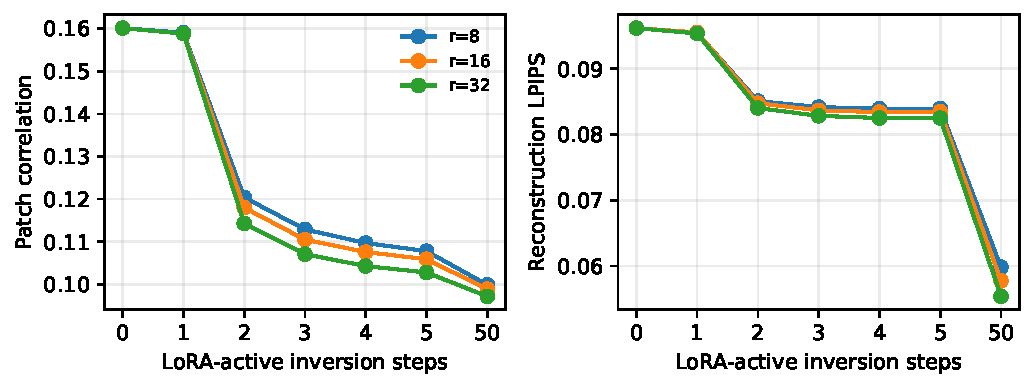
\includegraphics[width=0.9\linewidth]{figures/inversion_active_steps.pdf}
    \caption{Recovered-noise correlation and reconstruction LPIPS as the number of LoRA-active inversion steps increases. The final point uses all 50 steps.}
    \label{fig:active-steps}
\end{figure}

\begin{table*}[t]
    \centering
    \scriptsize
    \caption{Inversion quality when LoRA is enabled for only the first $k$ inversion steps. All entries are means.}
    \label{tab:lora-rank-window-comparison}
    \resizebox{\textwidth}{!}{%
    \begin{tabular}{llrrrrrr}
        \toprule
        Adapter & Steps & Corr. $\downarrow$ & KL $\times10^2$ $\downarrow$ & MAE $\downarrow$ & LPIPS $\downarrow$ & PSNR $\uparrow$ & SSIM $\uparrow$ \\
        \midrule
        None & 0 & 0.1601 & 0.8566 & 0.02663 & 0.09617 & 28.32 & 0.8112 \\
        \midrule
        $r=8$ & 1 & 0.1590 & 0.8499 & 0.02654 & 0.09546 & 28.34 & 0.8123 \\
        $r=8$ & 2 & 0.1204 & 0.3891 & 0.02508 & 0.08507 & 28.65 & 0.8304 \\
        $r=8$ & 3 & 0.1129 & 0.3007 & 0.02489 & 0.08416 & 28.70 & 0.8337 \\
        $r=8$ & 4 & 0.1097 & 0.2582 & 0.02482 & 0.08391 & 28.71 & 0.8349 \\
        $r=8$ & 5 & 0.1078 & 0.2327 & 0.02481 & 0.08393 & 28.71 & 0.8353 \\
        $r=8$ & 50 & 0.0999 & 0.0767 & 0.02063 & 0.05982 & 30.06 & 0.8654 \\
        \midrule
        $r=16$ & 1 & 0.1588 & 0.8499 & 0.02654 & 0.09551 & 28.34 & 0.8122 \\
        $r=16$ & 2 & 0.1180 & 0.3584 & 0.02508 & 0.08475 & 28.64 & 0.8312 \\
        $r=16$ & 3 & 0.1105 & 0.2687 & 0.02486 & 0.08366 & 28.69 & 0.8347 \\
        $r=16$ & 4 & 0.1076 & 0.2302 & 0.02479 & 0.08340 & 28.71 & 0.8359 \\
        $r=16$ & 5 & 0.1059 & 0.2075 & 0.02478 & 0.08346 & 28.70 & 0.8363 \\
        $r=16$ & 50 & 0.0989 & 0.0671 & 0.02028 & 0.05774 & 30.22 & 0.8699 \\
        \midrule
        $r=32$ & 1 & 0.1588 & 0.8486 & 0.02653 & 0.09536 & 28.34 & 0.8124 \\
        $r=32$ & 2 & 0.1143 & 0.3397 & 0.02497 & 0.08402 & 28.67 & 0.8325 \\
        $r=32$ & 3 & 0.1071 & 0.2502 & 0.02474 & 0.08283 & 28.72 & 0.8363 \\
        $r=32$ & 4 & 0.1043 & 0.2096 & 0.02466 & 0.08250 & 28.74 & 0.8377 \\
        $r=32$ & 5 & 0.1028 & 0.1861 & 0.02463 & 0.08249 & 28.74 & 0.8382 \\
        $r=32$ & 50 & \textbf{0.0972} & \textbf{0.0504} & \textbf{0.01970} & \textbf{0.05538} & \textbf{30.40} & \textbf{0.8743} \\
        \bottomrule
    \end{tabular}}
\end{table*}

\begin{table}[h]
    \centering
    \small
    \caption{Fraction of the full-trajectory improvement obtained with five active steps.}
    \label{tab:first-steps-share}
    \begin{tabular}{lrrrr}
        \toprule
        Metric & $r=8$ & $r=16$ & $r=32$ & Mean \\
        \midrule
        Corr. & 86.9\% & 88.4\% & 91.1\% & 88.8\% \\
        KL $\times10^2$ & 80.0\% & 82.2\% & 83.2\% & 81.8\% \\
        MAE & 30.4\% & 29.2\% & 28.8\% & 29.5\% \\
        LPIPS & 33.7\% & 33.1\% & 33.6\% & 33.4\% \\
        CLIP source & 69.5\% & 70.7\% & 73.2\% & 71.1\% \\
        CLIP target & 81.7\% & 81.2\% & 82.7\% & 81.9\% \\
        Directional CLIP & 88.4\% & 88.0\% & 91.9\% & 89.5\% \\
        \bottomrule
    \end{tabular}
\end{table}

\subsection{Plain and structured regions}
\begin{table*}[t]
    \centering
    \scriptsize
    \caption{Recovered-noise error and latent standard deviation in visually plain and non-plain regions. Values closer to $1$ indicate better agreement with the unit-Gaussian diffusion prior.}
    \label{tab:plain-nonplain}
    \resizebox{\textwidth}{!}{%
    \begin{tabular}{llrrrr}
        \toprule
        Adapter & Steps & Plain error $\downarrow$ & Non-plain error $\downarrow$ & Plain noise std. $\to1$ & Non-plain noise std. $\to1$ \\
        \midrule
        None & 0 & 0.1956 & 0.1682 & 0.8770 & 0.9573 \\
        $r=8$ & 1 & 0.1937 & 0.1667 & 0.8773 & 0.9576 \\
        $r=8$ & 2 & 0.1305 & 0.1204 & 0.9082 & 0.9750 \\
        $r=8$ & 3 & 0.1196 & 0.1120 & 0.9162 & 0.9801 \\
        $r=8$ & 4 & 0.1148 & 0.1083 & 0.9203 & 0.9830 \\
        $r=8$ & 5 & 0.1121 & 0.1061 & 0.9230 & 0.9849 \\
        $r=8$ & 50 & 0.1015 & 0.0970 & 0.9433 & 1.0022 \\
        \midrule
        $r=16$ & 1 & 0.1937 & 0.1667 & 0.8773 & 0.9576 \\
        $r=16$ & 2 & 0.1267 & 0.1175 & 0.9104 & 0.9764 \\
        $r=16$ & 3 & 0.1155 & 0.1088 & 0.9188 & 0.9819 \\
        $r=16$ & 4 & 0.1109 & 0.1052 & 0.9228 & 0.9847 \\
        $r=16$ & 5 & 0.1083 & 0.1031 & 0.9252 & 0.9865 \\
        $r=16$ & 50 & 0.0982 & 0.0944 & 0.9442 & 1.0029 \\
        \midrule
        $r=32$ & 1 & 0.1934 & 0.1664 & 0.8774 & 0.9576 \\
        $r=32$ & 2 & 0.1222 & 0.1140 & 0.9122 & 0.9776 \\
        $r=32$ & 3 & 0.1107 & 0.1052 & 0.9208 & 0.9832 \\
        $r=32$ & 4 & 0.1058 & 0.1014 & 0.9251 & 0.9862 \\
        $r=32$ & 5 & 0.1031 & 0.0992 & 0.9278 & 0.9882 \\
        $r=32$ & 50 & \textbf{0.0930} & \textbf{0.0906} & \textbf{0.9479} & 1.0055 \\
        \bottomrule
    \end{tabular}}
\end{table*}

\subsection{Synthetic text-editing probe}
For this controlled probe, each recovered latent is regenerated with a target prompt obtained by cyclically shifting the held-out source-prompt list. Lower CLIP source together with higher CLIP target and directional CLIP indicates greater responsiveness to the target condition. Table~\ref{tab:clip-editing-ablation} shows that most of the gain again appears in the first two to five corrected steps.
\begin{table*}[t]
    \centering
    \scriptsize
    \caption{CLIP metrics for the synthetic target-prompt probe. }
    \label{tab:clip-editing-ablation}
    \begin{tabular}{llrrr}
        \toprule
        Adapter & Steps & CLIP source $\downarrow$ & CLIP target $\uparrow$ & Directional CLIP $\uparrow$ \\
        \midrule
        None & 0 & 35.08 & 67.90 & 29.85 \\
        $r=8$ & 1 & 35.09 & 67.88 & 29.85 \\
        $r=8$ & 2 & 33.84 & 70.10 & 31.22 \\
        $r=8$ & 3 & 33.45 & 70.74 & 31.53 \\
        $r=8$ & 4 & 33.12 & 71.07 & 31.71 \\
        $r=8$ & 5 & 32.99 & 71.29 & 31.80 \\
        $r=8$ & 50 & 32.07 & 72.05 & 32.05 \\
        \midrule
        $r=16$ & 1 & 35.07 & 67.89 & 29.86 \\
        $r=16$ & 2 & 33.75 & 70.24 & 31.29 \\
        $r=16$ & 3 & 33.35 & 70.82 & 31.59 \\
        $r=16$ & 4 & 33.07 & 71.21 & 31.77 \\
        $r=16$ & 5 & 32.93 & 71.33 & 31.82 \\
        $r=16$ & 50 & 32.04 & 72.13 & \textbf{32.09} \\
        \midrule
        $r=32$ & 1 & 35.09 & 67.89 & 29.85 \\
        $r=32$ & 2 & 33.75 & 70.24 & 31.29 \\
        $r=32$ & 3 & 33.24 & 70.92 & 31.64 \\
        $r=32$ & 4 & 33.02 & 71.29 & 31.80 \\
        $r=32$ & 5 & 32.83 & 71.42 & 31.89 \\
        $r=32$ & 50 & \textbf{32.00} & \textbf{72.16} & 32.07 \\
        \bottomrule
    \end{tabular}
\end{table*}

\section{Guidance-scale robustness}
Applying the CFG-$1$ adapter at larger inversion guidance preserves latent normality initially but sharply damages reconstruction (Table~\ref{tab:cfg-sweep}). This motivates training against the actual conditional/unconditional branches used at the target CFG rather than treating a CFG-$1$ adapter as guidance-agnostic.
\begin{table}[h]
    \centering
    \small
    \caption{Applying the $r=32$ adapter at different inversion CFG values. All entries are means.}
    \label{tab:cfg-sweep}
    \resizebox{\linewidth}{!}{%
    \begin{tabular}{lrrrrrrr}
        \toprule
        Method & CFG & Corr. $\downarrow$ & KL $\times10^2$ $\downarrow$ & MAE $\downarrow$ & LPIPS $\downarrow$ & PSNR $\uparrow$ & SSIM $\uparrow$ \\
        \midrule
        DDIM Inv. & 1 & 0.1601 & 0.8566 & 0.02663 & 0.09617 & 28.32 & 0.8112 \\
        LoRA $r=32$ & 1 & 0.0972 & 0.0504 & \textbf{0.01970} & \textbf{0.05538} & \textbf{30.40} & \textbf{0.8743} \\
        LoRA $r=32$ & 2 & \textbf{0.0955} & \textbf{0.0150} & 0.07249 & 0.29056 & 21.16 & 0.6442 \\
        LoRA $r=32$ & 3 & 0.0989 & 0.0607 & 0.26066 & 0.64225 & 11.36 & 0.3292 \\
        LoRA $r=32$ & 4 & 0.1124 & 0.1500 & 0.32729 & 0.72783 & 9.10 & 0.2355 \\
        LoRA $r=32$ & 5 & 0.1331 & 0.2499 & 0.34274 & 0.75096 & 8.52 & 0.2063 \\
        \bottomrule
    \end{tabular}}
\end{table}

\begin{table}[h]
    \centering
    \small
    \caption{CFG-$4$ inversion on CFG-$4$ generated data (100-sample diagnostic). Noise standard deviation is a recovered-latent metric, not an uncertainty term.}
    \label{tab:cfg4-diagnostic}
    \resizebox{\linewidth}{!}{%
    \begin{tabular}{lrrrrrrr}
        \toprule
        Method & Noise std. $\to1$ & Corr. $\downarrow$ & KL $\downarrow$ & MAE $\downarrow$ & LPIPS $\downarrow$ & PSNR $\uparrow$ & SSIM $\uparrow$ \\
        \midrule
        DDIM Inv. & 0.8812 & 0.3669 & 2.2262 & 0.1725 & 0.5900 & 13.76 & 0.3566 \\
        Shared LoRA & \textbf{0.9828} & \textbf{0.3599} & \textbf{0.0838} & \textbf{0.0557} & \textbf{0.1939} & \textbf{22.09} & \textbf{0.7522} \\
        Branch-pair LoRA & 0.9562 & 0.3611 & 0.3306 & 0.0737 & 0.2489 & 20.40 & 0.7026 \\
        \bottomrule
    \end{tabular}}
\end{table}
\section{Cycle-consistency strength}
\label{sec:cycle-lambda-sweep}
Table~\ref{tab:cycle-lambda-sweep} reports the complete rank-16 cycle-weight sweep. P2P benefits most from a small cycle weight, with $\lambda_{\mathrm{cycle}}=0.5$ giving the strongest preservation. PnP is nearly insensitive to the tested range. For MasaCtrl, changing $\lambda_{\mathrm{cycle}}$ does not close the preservation gap to DirectInv, although several settings improve CLIP alignment. DirectInv remains stronger than every rank-16 cycle setting for Pix2Pix-Zero, indicating that cycle strength alone does not resolve that editor's inversion--attention mismatch.

\begin{table*}[p]
  \centering
  \scriptsize
  \setlength{\tabcolsep}{2.2pt}
  \renewcommand{\arraystretch}{0.90}
  \caption{Complete cycle-loss sweep for rank-16 LoRA+DirectInv on PIE-Bench. Bold denotes the best result within each editor, including the reproduced SD1.5 DirectInv control. Italics denote the best cycle-loss setting for each metric.}
  \label{tab:cycle-lambda-sweep}
  \resizebox{\textwidth}{!}{%
  \begin{tabular}{llrrrrrrr}
    \toprule
    Editor & $\lambda_{\mathrm{cycle}}$ &
    Structure ($\times 10^3$) $\downarrow$ & PSNR $\uparrow$ &
    LPIPS ($\times 10^3$) $\downarrow$ & MSE ($\times 10^4$) $\downarrow$ &
    SSIM ($\times 10^2$) $\uparrow$ & CLIP target $\uparrow$ &
    CLIP edit $\uparrow$ \\
    \midrule
    P2P & DirectInv & 31.35 & 22.57 & 125.51 & 91.27 & 78.54 & 25.07 & 22.22 \\
    P2P & 0.5 & \textbf{\textit{14.00}} & \textbf{\textit{26.05}} & \textbf{\textit{71.76}} & \textbf{\textit{43.57}} & \textbf{\textit{83.60}} & 25.28 & 22.31 \\
    P2P & 1 & 14.45 & 25.92 & 74.51 & 45.37 & 83.37 & 25.27 & 22.31 \\
    P2P & 2 & 14.41 & 25.92 & 74.10 & 44.87 & 83.39 & \textbf{\textit{25.32}} & \textbf{\textit{22.36}} \\
    P2P & 4 & 14.23 & 26.04 & 73.38 & 44.43 & 83.44 & \textbf{\textit{25.32}} & 22.30 \\
    P2P & 8 & 14.36 & 25.95 & 73.39 & 44.87 & 83.45 & \textbf{\textit{25.32}} & 22.32 \\
    P2P & 16 & 14.24 & 26.01 & 72.52 & 43.61 & 83.56 & 25.31 & 22.31 \\
    \midrule
    PnP & DirectInv & \textbf{23.33} & \textbf{22.46} & \textbf{105.51} & \textbf{79.97} & \textbf{80.22} & 25.63 & 22.67 \\
    PnP & 0.5 & \textit{24.38} & \textit{22.36} & 110.27 & 81.87 & \textit{79.88} & 25.81 & \textbf{\textit{22.83}} \\
    PnP & 1 & \textit{24.38} & \textit{22.36} & 110.28 & 81.87 & \textit{79.88} & 25.81 & \textbf{\textit{22.83}} \\
    PnP & 2 & \textit{24.38} & \textit{22.36} & 110.27 & 81.87 & \textit{79.88} & 25.81 & \textbf{\textit{22.83}} \\
    PnP & 4 & \textit{24.38} & \textit{22.36} & 110.27 & 81.87 & \textit{79.88} & 25.81 & 22.82 \\
    PnP & 8 & 24.39 & \textit{22.36} & 110.26 & 81.86 & \textit{79.88} & \textbf{\textit{25.82}} & \textbf{\textit{22.83}} \\
    PnP & 16 & 24.39 & \textit{22.36} & \textit{110.25} & \textit{81.85} & \textit{79.88} & 25.81 & \textbf{\textit{22.83}} \\
    \midrule
    MasaCtrl & DirectInv & \textbf{23.57} & \textbf{22.82} & \textbf{86.83} & \textbf{79.19} & \textbf{82.02} & 24.51 & 21.47 \\
    MasaCtrl & 0.5 & 28.52 & 21.89 & 98.93 & 99.02 & 80.50 & 24.61 & 21.47 \\
    MasaCtrl & 1 & 28.49 & 21.89 & 98.91 & 98.95 & 80.50 & \textbf{\textit{24.63}} & 21.48 \\
    MasaCtrl & 2 & 28.53 & \textit{21.90} & 98.83 & 99.05 & 80.50 & 24.62 & \textbf{\textit{21.50}} \\
    MasaCtrl & 4 & 28.51 & \textit{21.90} & 98.89 & \textit{98.91} & 80.50 & 24.62 & \textbf{\textit{21.50}} \\
    MasaCtrl & 8 & \textit{28.47} & \textit{21.90} & \textit{98.77} & \textit{98.91} & \textit{80.52} & 24.59 & 21.47 \\
    MasaCtrl & 16 & 28.49 & 21.89 & 98.88 & \textit{98.91} & 80.50 & \textbf{\textit{24.63}} & \textbf{\textit{21.50}} \\
    \midrule
    Pix2Pix-Zero & DirectInv & \textbf{49.99} & \textbf{21.47} & \textbf{142.46} & \textbf{133.49} & \textbf{77.49} & \textbf{23.53} & \textbf{21.09} \\
    Pix2Pix-Zero & 0.5 & 52.67 & 21.26 & 145.88 & 138.21 & 77.07 & \textit{23.43} & 21.04 \\
    Pix2Pix-Zero & 1 & 52.16 & 21.22 & 147.00 & 140.33 & 76.95 & \textit{23.43} & 20.98 \\
    Pix2Pix-Zero & 2 & 53.06 & 21.25 & 146.22 & 139.69 & 76.97 & 23.33 & 20.87 \\
    Pix2Pix-Zero & 4 & 52.06 & 21.27 & 146.70 & 139.76 & 77.02 & 23.41 & \textit{21.08} \\
    Pix2Pix-Zero & 8 & 52.38 & \textit{21.29} & 146.18 & 139.26 & 77.03 & \textit{23.43} & 20.93 \\
    Pix2Pix-Zero & 16 & \textit{51.41} & 21.26 & \textit{145.77} & \textit{137.38} & \textit{77.12} & 23.33 & 20.89 \\
    \bottomrule
  \end{tabular}}
\end{table*}


\begin{table}[t]
\centering\scriptsize
\caption{Reconstruction quality and edit alignment of DDIM and mixed-CFG-trained
LoRA variants with equal inversion and generation CFG. MSE, MAE and CLIP-S
are minimized; PSNR, SSIM, CLIP-T and Dir. CLIP are maximized. All results
are means. Bold denotes the best reported result within each CFG setting.}
\label{tab:cfg-matched-mixed}
\resizebox{\linewidth}{!}{%
\begin{tabular}{llrrrrrrr}
        \toprule
        $w_{\rm inv}=w_{\rm gen}$ & Inversion & MSE $\downarrow$ & MAE $\downarrow$ & PSNR $\uparrow$ & SSIM $\uparrow$ &
        CLIP-S $\downarrow$ & CLIP-T $\uparrow$ & Dir. CLIP $\uparrow$ \\
        \midrule
        2.0 & DDIM & 0.00827 & 0.0561 & 23.16 & 0.6563 & 33.49 & 74.08 & 34.08 \\
            & Shared CFG & \textbf{0.00347} & \textbf{0.0341} & \textbf{26.09} & \textbf{0.8149} & 30.14 & 80.20 & \textbf{36.94} \\
            & Shared branch & 0.00355 & 0.0349 & 25.61 & 0.8075 & \textbf{29.67} & \textbf{80.47} & 36.93 \\
            & Pair CFG & 0.02803 & 0.1352 & 15.70 & 0.5356 & 39.88 & 40.02 & 18.29 \\
            & Pair branch & 0.00531 & 0.0460 & 23.71 & 0.7347 & 29.85 & 79.80 & 36.79 \\
        \midrule
        3.0 & DDIM & 0.03172 & 0.1248 & 16.76 & 0.4171 & 35.83 & 72.24 & 32.61 \\
            & Shared CFG & \textbf{0.00613} & \textbf{0.0427} & \textbf{24.49} & \textbf{0.7952} & 29.60 & 81.94 & 37.81 \\
            & Shared branch & 0.00758 & 0.0503 & 22.76 & 0.7687 & \textbf{28.80} & \textbf{82.36} & \textbf{37.97} \\
            & Pair CFG & 0.02984 & 0.1374 & 15.44 & 0.5448 & 39.23 & 40.15 & 19.23 \\
            & Pair branch & 0.01657 & 0.0792 & 19.99 & 0.6474 & 30.06 & 80.47 & 36.98 \\
        \midrule
        4.0 & DDIM & 0.05467 & 0.1736 & 13.68 & 0.3464 & 36.72 & 67.66 & 30.82 \\
            & Shared CFG & \textbf{0.01351} & \textbf{0.0658} & \textbf{21.40} & \textbf{0.7392} & \textbf{28.76} & 82.58 & 38.40 \\
            & Shared branch & 0.01616 & 0.0764 & 19.77 & 0.6985 & 28.78 & \textbf{83.37} & \textbf{38.60} \\
            & Pair CFG & 0.03115 & 0.1373 & 15.26 & 0.5440 & 40.15 & 43.05 & 20.54 \\
            & Pair branch & 0.04813 & 0.1477 & 15.48 & 0.5134 & 30.88 & 77.53 & 36.03 \\
        \midrule
        5.0 & DDIM & 0.07277 & 0.2047 & 12.07 & 0.3355 & 36.02 & 64.94 & 30.04 \\
            & Shared CFG & \textbf{0.02578} & \textbf{0.0977} & \textbf{18.49} & \textbf{0.6567} & 29.48 & 81.98 & 38.13 \\
            & Shared branch & 0.03562 & 0.1221 & 16.33 & 0.5979 & \textbf{29.24} & \textbf{82.74} & \textbf{38.28} \\
            & Pair CFG & 0.03417 & 0.1413 & 14.89 & 0.5414 & 39.74 & 48.14 & 22.66 \\
            & Pair branch & 0.09919 & 0.2389 & 11.30 & 0.3538 & 33.69 & 69.37 & 32.19 \\
        \midrule
        7.5 & DDIM & 0.10139 & 0.2468 & 10.30 & 0.3163 & 37.10 & 60.04 & 28.53 \\
            & Shared CFG & 0.06526 & 0.1767 & 13.39 & 0.5101 & \textbf{30.94} & \textbf{77.90} & \textbf{36.70} \\
            & Shared branch & 0.10671 & 0.2462 & 10.62 & 0.3962 & 32.53 & 71.98 & 33.87 \\
            & Pair CFG & \textbf{0.04216} & \textbf{0.1552} & \textbf{14.01} & \textbf{0.5401} & 38.92 & 69.17 & 30.96 \\
            & Pair branch & 0.18254 & 0.3574 & 7.52 & 0.1869 & 37.73 & 51.68 & 24.42 \\
        \midrule
        10.0 & DDIM & 0.12182 & 0.2711 & 9.37 & 0.2946 & 37.99 & 55.59 & 26.80 \\
             & Shared CFG & 0.11570 & 0.2603 & 9.78 & \textbf{0.3787} & \textbf{34.58} & 68.99 & \textbf{32.48} \\
             & Shared branch & 0.15604 & 0.3131 & 8.37 & 0.2888 & 35.92 & 62.21 & 29.44 \\
             & Pair CFG & \textbf{0.09063} & \textbf{0.2320} & \textbf{10.72} & 0.3506 & 40.19 & \textbf{70.83} & 30.83 \\
             & Pair branch & 0.19553 & 0.3669 & 7.15 & 0.1688 & 37.75 & 45.89 & 22.54 \\
        \bottomrule
    \end{tabular}}
\end{table}



\begin{table}[t]
\centering\scriptsize
\caption{Inversion quality and edit alignment of DDIM and guided LoRA variants.
Correlation, KL divergence and LPIPS are minimized; PSNR, SSIM and CLIP
scores are maximized. All results are means. Bold denotes the best reported
mean within each generation-guidance setting.}
\label{tab:cfg-common-r16}
\resizebox{\linewidth}{!}{%
\begin{tabular}{rlrrrrrrr}
\toprule
CFG gen. & Inversion & Corr. $\downarrow$ & KL $\downarrow$ &
LPIPS $\downarrow$ & PSNR $\uparrow$ & SSIM $\uparrow$ &
CLIP-T $\uparrow$ & Dir. CLIP $\uparrow$ \\
\midrule
5 & DDIM & 0.18093 & 2.42355 & 0.18965 & 19.89 & 0.7444 & 80.50 & 37.17 \\
 & Single-pass & 0.12247 & 0.21056 & 0.18793 & 19.77 & 0.7482 & 84.28 & 39.03 \\
 & Shared CFG & \textbf{0.11746} & \textbf{0.03973} & 0.18818 & 19.91 & 0.7468 & \textbf{84.60} & \textbf{39.08} \\
 & Shared branch & 0.12135 & 0.23944 & \textbf{0.17634} & \textbf{20.31} & \textbf{0.7612} & 84.04 & 39.00 \\
 & Pair CFG & 0.11895 & 0.13086 & 0.21203 & 19.31 & 0.7261 & 84.23 & 38.93 \\
 & Pair branch & 0.12108 & 0.19438 & 0.17797 & 20.27 & 0.7595 & 84.20 & 38.99 \\
\midrule
7.5 & DDIM & 0.18670 & 2.85674 & 0.22280 & 17.73 & 0.6931 & 81.76 & 37.97 \\
 & Single-pass & 0.12402 & 0.26300 & 0.21872 & 17.79 & 0.6975 & 85.04 & 39.62 \\
 & Shared CFG & \textbf{0.11798} & \textbf{0.04718} & 0.22357 & 17.81 & 0.6918 & \textbf{85.36} & 39.59 \\
 & Shared branch & 0.12282 & 0.30069 & \textbf{0.20854} & \textbf{18.17} & \textbf{0.7095} & 85.27 & \textbf{39.69} \\
 & Pair CFG & 0.11960 & 0.13733 & 0.24335 & 17.35 & 0.6748 & 85.23 & 39.61 \\
 & Pair branch & 0.12257 & 0.25404 & 0.21113 & 18.13 & 0.7078 & 85.17 & 39.60 \\
\midrule
10 & DDIM & 0.19018 & 3.12596 & 0.25287 & 16.30 & 0.6473 & 82.12 & 38.16 \\
 & Single-pass & 0.12523 & 0.30958 & 0.24565 & 16.44 & 0.6507 & 85.40 & \textbf{39.84} \\
 & Shared CFG & \textbf{0.11833} & \textbf{0.05570} & 0.25186 & 16.41 & 0.6448 & \textbf{85.75} & \textbf{39.84} \\
 & Shared branch & 0.12400 & 0.35233 & \textbf{0.23606} & \textbf{16.74} & \textbf{0.6620} & 85.21 & 39.75 \\
 & Pair CFG & 0.12022 & 0.14363 & 0.27316 & 15.94 & 0.6267 & 85.57 & 39.79 \\
 & Pair branch & 0.12368 & 0.30700 & 0.23881 & 16.71 & 0.6606 & 85.43 & 39.79 \\
\bottomrule
\end{tabular}}
\end{table}



\begin{table}[t]
 \centering\small
 \caption{Effect of separating inversion and generation guidance for DDIM.
 LPIPS is minimized; PSNR, SSIM and CLIP scores are maximized.
 All results are means. Bold denotes the best result within each
 generation-guidance setting.}
 \label{tab:high-cfg-ablation}
 \resizebox{\linewidth}{!}{%
 \begin{tabular}{rrlrrrrr}
 \toprule
 CFG inv. & CFG gen. & Inversion & LPIPS $\downarrow$ & PSNR $\uparrow$ & SSIM $\uparrow$ & CLIP-T $\uparrow$ & Dir. CLIP $\uparrow$ \\
 \midrule
 5 & 5 & DDIM & 0.6285 & 12.07 & 0.3355 & 64.94 & 30.04 \\
 2 & 5 & DDIM & \textbf{0.1871} & \textbf{20.07} & \textbf{0.7450} & \textbf{80.10} & \textbf{37.08} \\
 7.5 & 7.5 & DDIM & 0.6484 & 10.30 & 0.3163 & 60.04 & 28.53 \\
 2 & 7.5 & DDIM & \textbf{0.2237} & \textbf{17.79} & \textbf{0.6899} & \textbf{82.10} & \textbf{38.21} \\
 10 & 10 & DDIM & 0.6670 & 9.37 & 0.2946 & 55.59 & 26.80 \\
 2 & 10 & DDIM & \textbf{0.2539} & \textbf{16.38} & \textbf{0.6429} & \textbf{81.92} & \textbf{38.62} \\
 \bottomrule
 \end{tabular}}
\end{table}


\begin{table}[t]
\centering\scriptsize
\caption{Noise diagnostics, reconstruction and editing quality for FLUX
inversion at different guidance settings. Correlation, KL divergence, MAE,
LPIPS and source CLIP are minimized; the remaining metrics are maximized.
All results are means. Bold denotes the best reported mean within each block.}
\label{tab:flux-synthetic-guidance}
\resizebox{\linewidth}{!}{%
\begin{tabular}{lrrrrrrrrr}
\toprule
Inversion & Corr. $\downarrow$ & KL $\downarrow$ & MAE $\downarrow$ &
LPIPS $\downarrow$ & PSNR $\uparrow$ & SSIM $\uparrow$ &
CLIP-S $\downarrow$ & CLIP-T $\uparrow$ & Dir. CLIP $\uparrow$ \\
\midrule
\multicolumn{10}{l}{$g_{\rm src}=g_{\rm inv}=g_{\rm rec}=g_{\rm edit}=1$} \\
Euler & 0.13795 & 0.3796 & 0.08970 & 0.50005 & 18.97 & 0.63897 & 33.949 & 78.456 & 33.486 \\
Nudging $\times1.5$ & 0.28697 & 6.1737 & 0.03841 & 0.17837 & 26.17 & 0.84902 & 63.451 & 47.924 & 15.849 \\
LoRA & \textbf{0.13650} & \textbf{0.0397} & \textbf{0.01733} & \textbf{0.07333} & \textbf{32.43} & \textbf{0.95713} & \textbf{32.033} & \textbf{80.378} & \textbf{34.845} \\
\midrule
\multicolumn{10}{l}{$g_{\rm src}=g_{\rm inv}=g_{\rm rec}=g_{\rm edit}=3.5$} \\
Euler & 0.18743 & 3.9522 & 0.21394 & 0.72322 & 11.20 & 0.43764 & \textbf{33.071} & \textbf{73.917} & \textbf{32.813} \\
Nudging $\times1.5$ & 0.37150 & 3.2313 & \textbf{0.06833} & \textbf{0.15837} & \textbf{22.93} & \textbf{0.80523} & 72.051 & 40.391 & 9.840 \\
LoRA & \textbf{0.14628} & \textbf{0.8322} & 0.26107 & 0.75262 & 9.47 & 0.39155 & 33.718 & 67.161 & 30.308 \\
\midrule
\multicolumn{10}{l}{$g_{\rm src}=g_{\rm rec}=g_{\rm edit}=3.5,\quad g_{\rm inv}=1$} \\
Euler & 0.17916 & 4.2695 & 0.06236 & 0.17645 & 20.85 & \textbf{0.81535} & 31.463 & 78.916 & 35.252 \\
Nudging $\times1.5$ & 0.36462 & 3.2371 & 0.09074 & \textbf{0.15229} & 19.56 & 0.78944 & 78.477 & 36.375 & 6.636 \\
LoRA & \textbf{0.14830} & \textbf{1.4746} & \textbf{0.06115} & 0.17746 & \textbf{20.97} & 0.80636 & \textbf{29.028} & \textbf{80.415} & \textbf{36.655} \\
\bottomrule
\end{tabular}}
\end{table}


\begin{table*}[t]
 \centering\scriptsize
 \setlength{\tabcolsep}{3pt}
 \caption{Full-image reconstruction, background preservation after editing,
 and edit alignment for FLUX on PIE-Bench. LPIPS, MSE and MAE are minimized;
 PSNR, SSIM and CLIP scores are maximized. All results are means.
 Bold denotes the best result in each column.}
 \label{tab:flux-pie}
 \resizebox{\textwidth}{!}{%
 \begin{tabular}{lrrrrrrrrrrr}
 \toprule
 & \multicolumn{5}{c}{Full-image reconstruction} &
 \multicolumn{4}{c}{Background after editing} & \multicolumn{2}{c}{CLIP-T} \\
 \cmidrule(lr){2-6}\cmidrule(lr){7-10}\cmidrule(lr){11-12}
 Inversion & PSNR $\uparrow$ & LPIPS $\downarrow$ & MSE $\downarrow$ & SSIM $\uparrow$ & MAE $\downarrow$ &
 PSNR $\uparrow$ & LPIPS $\downarrow$ & MSE $\downarrow$ & SSIM $\uparrow$ & Whole $\uparrow$ & Mask $\uparrow$ \\
 \midrule
 Euler & 16.88 & 329.96 & 284.88 & 60.14 & 0.11741 & 17.28 & 245.79 & 281.38 & 69.99 & 23.68 & 21.44 \\
 LoRA & 20.95 & 194.15 & 180.07 & 75.42 & 0.07561 & 18.59 & 197.14 & 257.52 & 75.98 & \textbf{24.33} & \textbf{21.73} \\
 Nudging $\times1.5$ & \textbf{22.10} & \textbf{82.27} & \textbf{115.19} & \textbf{79.11} & \textbf{0.06248} &
 \textbf{23.55} & \textbf{67.29} & \textbf{101.47} & \textbf{84.94} & 23.20 & 20.38 \\
 \bottomrule
 \end{tabular}}
\end{table*}



\clearpage
\begin{figure}[p]
 \centering
\begingroup
\setlength{\tabcolsep}{1pt}
\renewcommand{\arraystretch}{0.96}
\begin{tabular}{@{}*{3}{c}@{}}
\parbox[c]{0.318\linewidth}{\centering\scriptsize\bfseries Style reference} & \parbox[c]{0.318\linewidth}{\centering\scriptsize\bfseries DDIM} & \parbox[c]{0.318\linewidth}{\centering\scriptsize\bfseries LoRA r16} \\
\multicolumn{3}{@{}l@{}}{\scriptsize (a) Target prompt: A person jogging along a scenic trail} \\[-1pt]
\includegraphics[width=0.318\linewidth,height=0.150\textheight,keepaspectratio]{figures/qualitative/appendix/instantstyle_s0_improvement/row_01_01_style_reference.jpg} & \includegraphics[width=0.318\linewidth,height=0.150\textheight,keepaspectratio]{figures/qualitative/appendix/instantstyle_s0_improvement/row_01_02_ddim.jpg} & \includegraphics[width=0.318\linewidth,height=0.150\textheight,keepaspectratio]{figures/qualitative/appendix/instantstyle_s0_improvement/row_01_03_lora_r16.jpg} \\[2pt]
\multicolumn{3}{@{}l@{}}{\scriptsize (b) Target prompt: A chef preparing meals in kitchen} \\[-1pt]
\includegraphics[width=0.318\linewidth,height=0.150\textheight,keepaspectratio]{figures/qualitative/appendix/instantstyle_s0_improvement/row_02_01_style_reference.jpg} & \includegraphics[width=0.318\linewidth,height=0.150\textheight,keepaspectratio]{figures/qualitative/appendix/instantstyle_s0_improvement/row_02_02_ddim.jpg} & \includegraphics[width=0.318\linewidth,height=0.150\textheight,keepaspectratio]{figures/qualitative/appendix/instantstyle_s0_improvement/row_02_03_lora_r16.jpg} \\[2pt]
\multicolumn{3}{@{}l@{}}{\scriptsize (c) Target prompt: A robot} \\[-1pt]
\includegraphics[width=0.318\linewidth,height=0.150\textheight,keepaspectratio]{figures/qualitative/appendix/instantstyle_s0_improvement/row_03_01_style_reference.jpg} & \includegraphics[width=0.318\linewidth,height=0.150\textheight,keepaspectratio]{figures/qualitative/appendix/instantstyle_s0_improvement/row_03_02_ddim.jpg} & \includegraphics[width=0.318\linewidth,height=0.150\textheight,keepaspectratio]{figures/qualitative/appendix/instantstyle_s0_improvement/row_03_03_lora_r16.jpg} \\[2pt]
\multicolumn{3}{@{}l@{}}{\scriptsize (c) Target prompt: A house with a tree beside} \\[-1pt]
\includegraphics[width=0.318\linewidth,height=0.150\textheight,keepaspectratio]{figures/qualitative/appendix/instantstyle_s0_improvement/row_04_01_style_reference.jpg} & \includegraphics[width=0.318\linewidth,height=0.150\textheight,keepaspectratio]{figures/qualitative/appendix/instantstyle_s0_improvement/row_04_02_ddim.jpg} & \includegraphics[width=0.318\linewidth,height=0.150\textheight,keepaspectratio]{figures/qualitative/appendix/instantstyle_s0_improvement/row_04_03_lora_r16.jpg} \\[2pt]
\multicolumn{3}{@{}l@{}}{\scriptsize (b) Target prompt: A student walking to school with backpack} \\[-1pt]
\includegraphics[width=0.318\linewidth,height=0.150\textheight,keepaspectratio]{figures/qualitative/appendix/instantstyle_s0_improvement/row_05_01_style_reference.jpg} & \includegraphics[width=0.318\linewidth,height=0.150\textheight,keepaspectratio]{figures/qualitative/appendix/instantstyle_s0_improvement/row_05_02_ddim.jpg} & \includegraphics[width=0.318\linewidth,height=0.150\textheight,keepaspectratio]{figures/qualitative/appendix/instantstyle_s0_improvement/row_05_03_lora_r16.jpg} \\[2pt]
\end{tabular}
\endgroup
 \caption{Inversion-InstantStyle at $s=0$.}
 \label{fig:qual-appendix-5}
\end{figure}
\clearpage



\end{document}




\end{document}
